Les deux projets de recherche, \enquote{La couleur~: artefacts, matière et cognition} et \enquote{La fabrique matérielle du visuel~: panneaux peints en Méditerranée}, ont chacune des entrées de leur base de données reliée à une image numérique. Il s'agit d'une photographie, en haute résolution, du feuillet de manuscrit ou du panneau qui est l'objet des analyses. Il y en a plus de mille cent. C'est un atout majeur du projet~: elles permettent non seulement de faire connaître au grand public des chefs-d'œuvre conservés dans les manuscrits, mais également de servir de supports aux analyses pour les chercheurs.\par
Le musée d’art et d'antiquités de l'université de Cambridge, le Fitzwilliam Museum, a proposé une valorisation de ses manuscrits enluminés à l'adresse suivante~: \url{https://www.fitzmuseum.cam.ac.uk/illuminated/}. À partir d'une petite sélection, les équipes du musée présentent les enluminures en haute résolution, avec des métadonnées descriptives et des points d'analyse sous forme d'annotations. Il me semble que le travail réalisé ici peut servir de modèle pour d'autres projets de recherche, comme ceux qui nous concernent aujourd'hui. Il est, d'une certaine façon, question de faire au cours de ce stage une démarche similaire avec des manuscrits sélectionnés par le département des manuscrits.\newpage

\section{Un fac-similé numérique}

L’idée est de travailler à partir des images numérisées des feuillets et de proposer des annotations qui pourront servir aux chercheurs. Une annotation est une information supplémentaire ajoutée à l'image, soit pour la décrire, soit pour y apporter des informations. Dans notre cas, il s’agit d’y renseigner les données de la base sur les analyses réalisées. Ces annotations se superposent à des images qui s’inscrivent dans un ensemble de protocoles, appelé IIIF.\par
L'International Image Interoperability Framework (IIIF) a été développé pour répondre à la nécessité d'un accès standardisé et interopérable aux images numériques dans le domaine des bibliothèques, archives et musées\footcite{noauthor_international_2024}. L’idée de ce consortium\footnote{Parmi les premières institutions à travailler sur les protocoles IIIF, nous pouvons citer la Bibliothèque Bodleian de l'Université d'Oxford, la Bibliothèque de l'Université de Stanford ou encore la British Library.}, fondé au cours de la décennie précédente, est de changer la manière dont les images numériques sont partagées et utilisées. Les images seront numérisées une seule fois en haute résolution par une institution, et elles seront déposées sur une plateforme, d’où elles pourront être appelées par n’importe quel utilisateur, selon son besoin spécifique. Ainsi, pour ce qui est des images des manuscrits que nous souhaitons valoriser, il suffit d’appeler les images numériques présentes sur la plateforme Gallica. L’interopérabilité permet de ne plus se soucier du processus de numérisation, déjà assuré par d’autres services.\\\par
Avec les protocoles qui définissent IIIF, les images sont non seulement consultables par n’importe quelle application ou logiciel compatible, mais elles sont également manipulables et annotables\footcite[La présentation de IIIF qui suit doit beaucoup à deux sites internet de vulgarisation. Le premier est le workbench de Glen Robson, le second est la documentation proposée Régis Robineau pour Biblissima][]{robson_iiif_nodate,biblissima_quest-ce_nodate}. Pour ce faire, il faut passer par des interfaces de programmation d’application (API). Dans le cadre de IIIF, ces dernières sont doubles. Elles concernent aussi bien l’image en elle-même, appelée l’API image, que sa présentation, c’est-à-dire avec ses métadonnées, appelée l’API présentation.\par
L’API image permet d’appeler les pixels d’une image et de manipuler cette dernière à distance à travers une syntaxe d’URL standardisée. Le modèle de toute API image suit ce schéma~:\par
{scheme}://{server}{/prefix}/{identifier}/{region}/{size}/{rotation}/{quality}.{format}\par
Pour les images que j’appelle sur Gallica pour les manifestes du projet, elles deviennent par exemple~:\par 
https://gallica.bnf.fr/iiif/ark:/1214/btv1b6000718s/f1/full/full/0/native.jpg\par
Il est dès lors possible de changer de région, de taille, de rotation, de qualité et de format selon les besoins spécifiques.\par
De son côté l’API présentation est décrite par Régis Robineau comme celle qui \enquote{spécifie les métadonnées (descriptives, structurelles, techniques) nécessaires à la présentation d’un objet numérique dans une interface. Toutes ces informations sont contenues dans un fichier appelé \enquote{manifeste}, une sorte d’enveloppe virtuelle formant l’unité de distribution élémentaire dans l’univers IIIF\footnote{https://doc.biblissima.fr/iiif/introduction-iiif/\#principe}. C’est en général ce fichier que vont manipuler les logiciels pour interagir avec une ressource, la visualiser, ou la transférer vers un autre outil.}\par
Un manifeste IIIF peut être un fac-similé numérique d’un objet physique (livre, manuscrit, périodique, carte, peinture, photographie, partition, monnaie, objet archéologique, archive sonore, captation vidéo, etc.), mais aussi un objet virtuel et composite constitué d’une série d’images ou d’autres médias rassemblés à des fins scientifiques ou pédagogiques, et pouvant provenir de différentes collections\footnote{https://doc.biblissima.fr/iiif/introduction-iiif/\#principe}. Dans le cas présent, les manifestes produits pour le stage s’apparentent à la première catégorie. Il s’agit d’un fac-similé numérique de manuscrit avec quelques annotations supplémentaires.\par
Le schéma ci-dessous, qui est proposé dans la documentation Biblissima, reprend les principales composantes d’un manifeste IIIF et permet de s’en faire une idée plus juste.

\begin{figure}[H]
	\centering
	\includegraphics[scale=0.19]{./textes/chap4/schema-iiif.jpg}
	\caption{Structure d'un manifeste IIIF}
	\label{fig:info}
\end{figure}

Les manifestes peuvent être affichés avec des visualiseurs IIIF. Ils proposent à l’utilisateur une expérience de \indexmot{visualisation} riche, s’appuyant sur l’ensemble des informations contenues dans les manifestes, au format JSON-LD. Les deux images ci-dessous permettent d’illustrer où sont mobilisées les deux API image et présentation dans un visualiseur comme Mirador~2. \par

\begin{figure}[H]
	\centering
	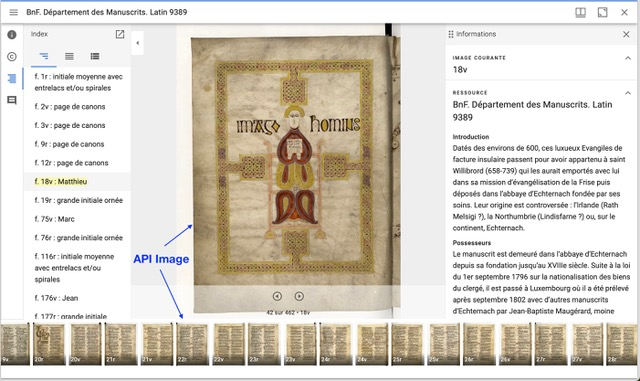
\includegraphics[scale=0.6]{./textes/chap4/mirador-api-image.jpeg}
	\caption{API Image}
	\label{fig:info}
\end{figure}
\begin{figure}[H]
	\centering
	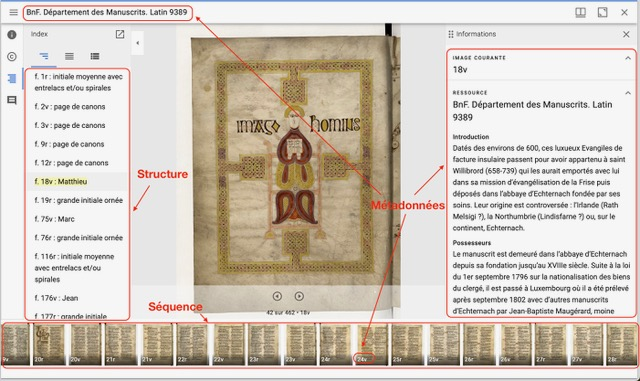
\includegraphics[scale=0.6]{./textes/chap4/mirador-api-presentation.jpeg}
	\caption{API Présentation}
	\label{fig:info}
\end{figure}

\newpage

\section{Enrichir une image numérique}

Les manifestes édités sont, je l’ai écrit précédemment, en quelque sorte un fac-similé numérique de manuscrit, avec quelques annotations supplémentaires. L’édition doit se faire au plus près de la version d’origine du manuscrit. Pour ce faire, et pour nos manuscrits, le point de départ est la bibliothèque numérique Gallica. La plateforme Gallica contient non seulement la numérisation de millions de documents de la \indexmot{Bibliothèque nationale de France}, mais elle donne également accès à une API qui permet de récupérer des manuscrits numérisés avec leur manifeste IIIF. Ces derniers permettent de récupérer tous les feuillets du document en haute résolution, ainsi que ses métadonnées descriptives et de séquences. Si je prends l’exemple du manuscrit Arabe~5847, Gallica propose l’intégralité de sa numérisation (avec les pages de couverture, pages de garde, contreplats et même le dos) dans le manifeste https://gallica.bnf.fr/iiif/ark:/12148/btv1b8422965p/manifest.json. Ce dernier contient également toutes les séquences du manuscrit, un titre pour tous les feuillets renseignés, qu’ils soient recto ou verso. Cette récupération auprès de Gallica permet de disposer du manuscrit Arabe~5847 en haute résolution et de travailler à la personnalisation du manifeste à partir de 9~292 lignes de JSON-LD déjà écrite par la plateforme.\par
Pour personnaliser le fac-similé numérique, il faut lui attribuer un nouvel identifiant unique. Chaque manifeste ne peut avoir qu’un seul identifiant. Pour différencier le travail qui sera réalisé sur le manuscrit de ce que propose Gallica, il convient donc de le rééditer sous un autre nom. La Bibliothèque Bodleian de l'Université d'Oxford met à la disposition du public un outil en ligne pour aider à la réédition. Il se trouve à l’adresse~: https://digital.bodleian.ox.ac.uk/manifest-editor/\#/?\_k=xjzu5x. L’éditeur permet de travailler soit à partir d’un nouveau manifeste, soit de reprendre un préexistant en le modifiant et en lui attribuant un nouvel identifiant. Dans notre cas, il suffit d’importer le canevas du manuscrit qui est renseigné sur Gallica. Ensuite, il est possible de personnaliser les métadonnées directement sur le site internet. Si les métadonnées descriptives de notre fac-similé numérique sont proches de celles de la plateforme de la BNF quant au titre, son introduction, son historique ou encore sa description technique, elles diffèrent au moment de les relier aux deux projets de recherche. Un paragraphe sur les matériaux utilisés dans le manuscrit est ainsi ajouté. En conséquence, lorsqu’une visionneuse IIIF interprétera le manifeste, il y aura, parmi les informations personnalisées, un premier résumé des résultats de la recherche.\newpage
\begin{figure}[H]
	\centering
	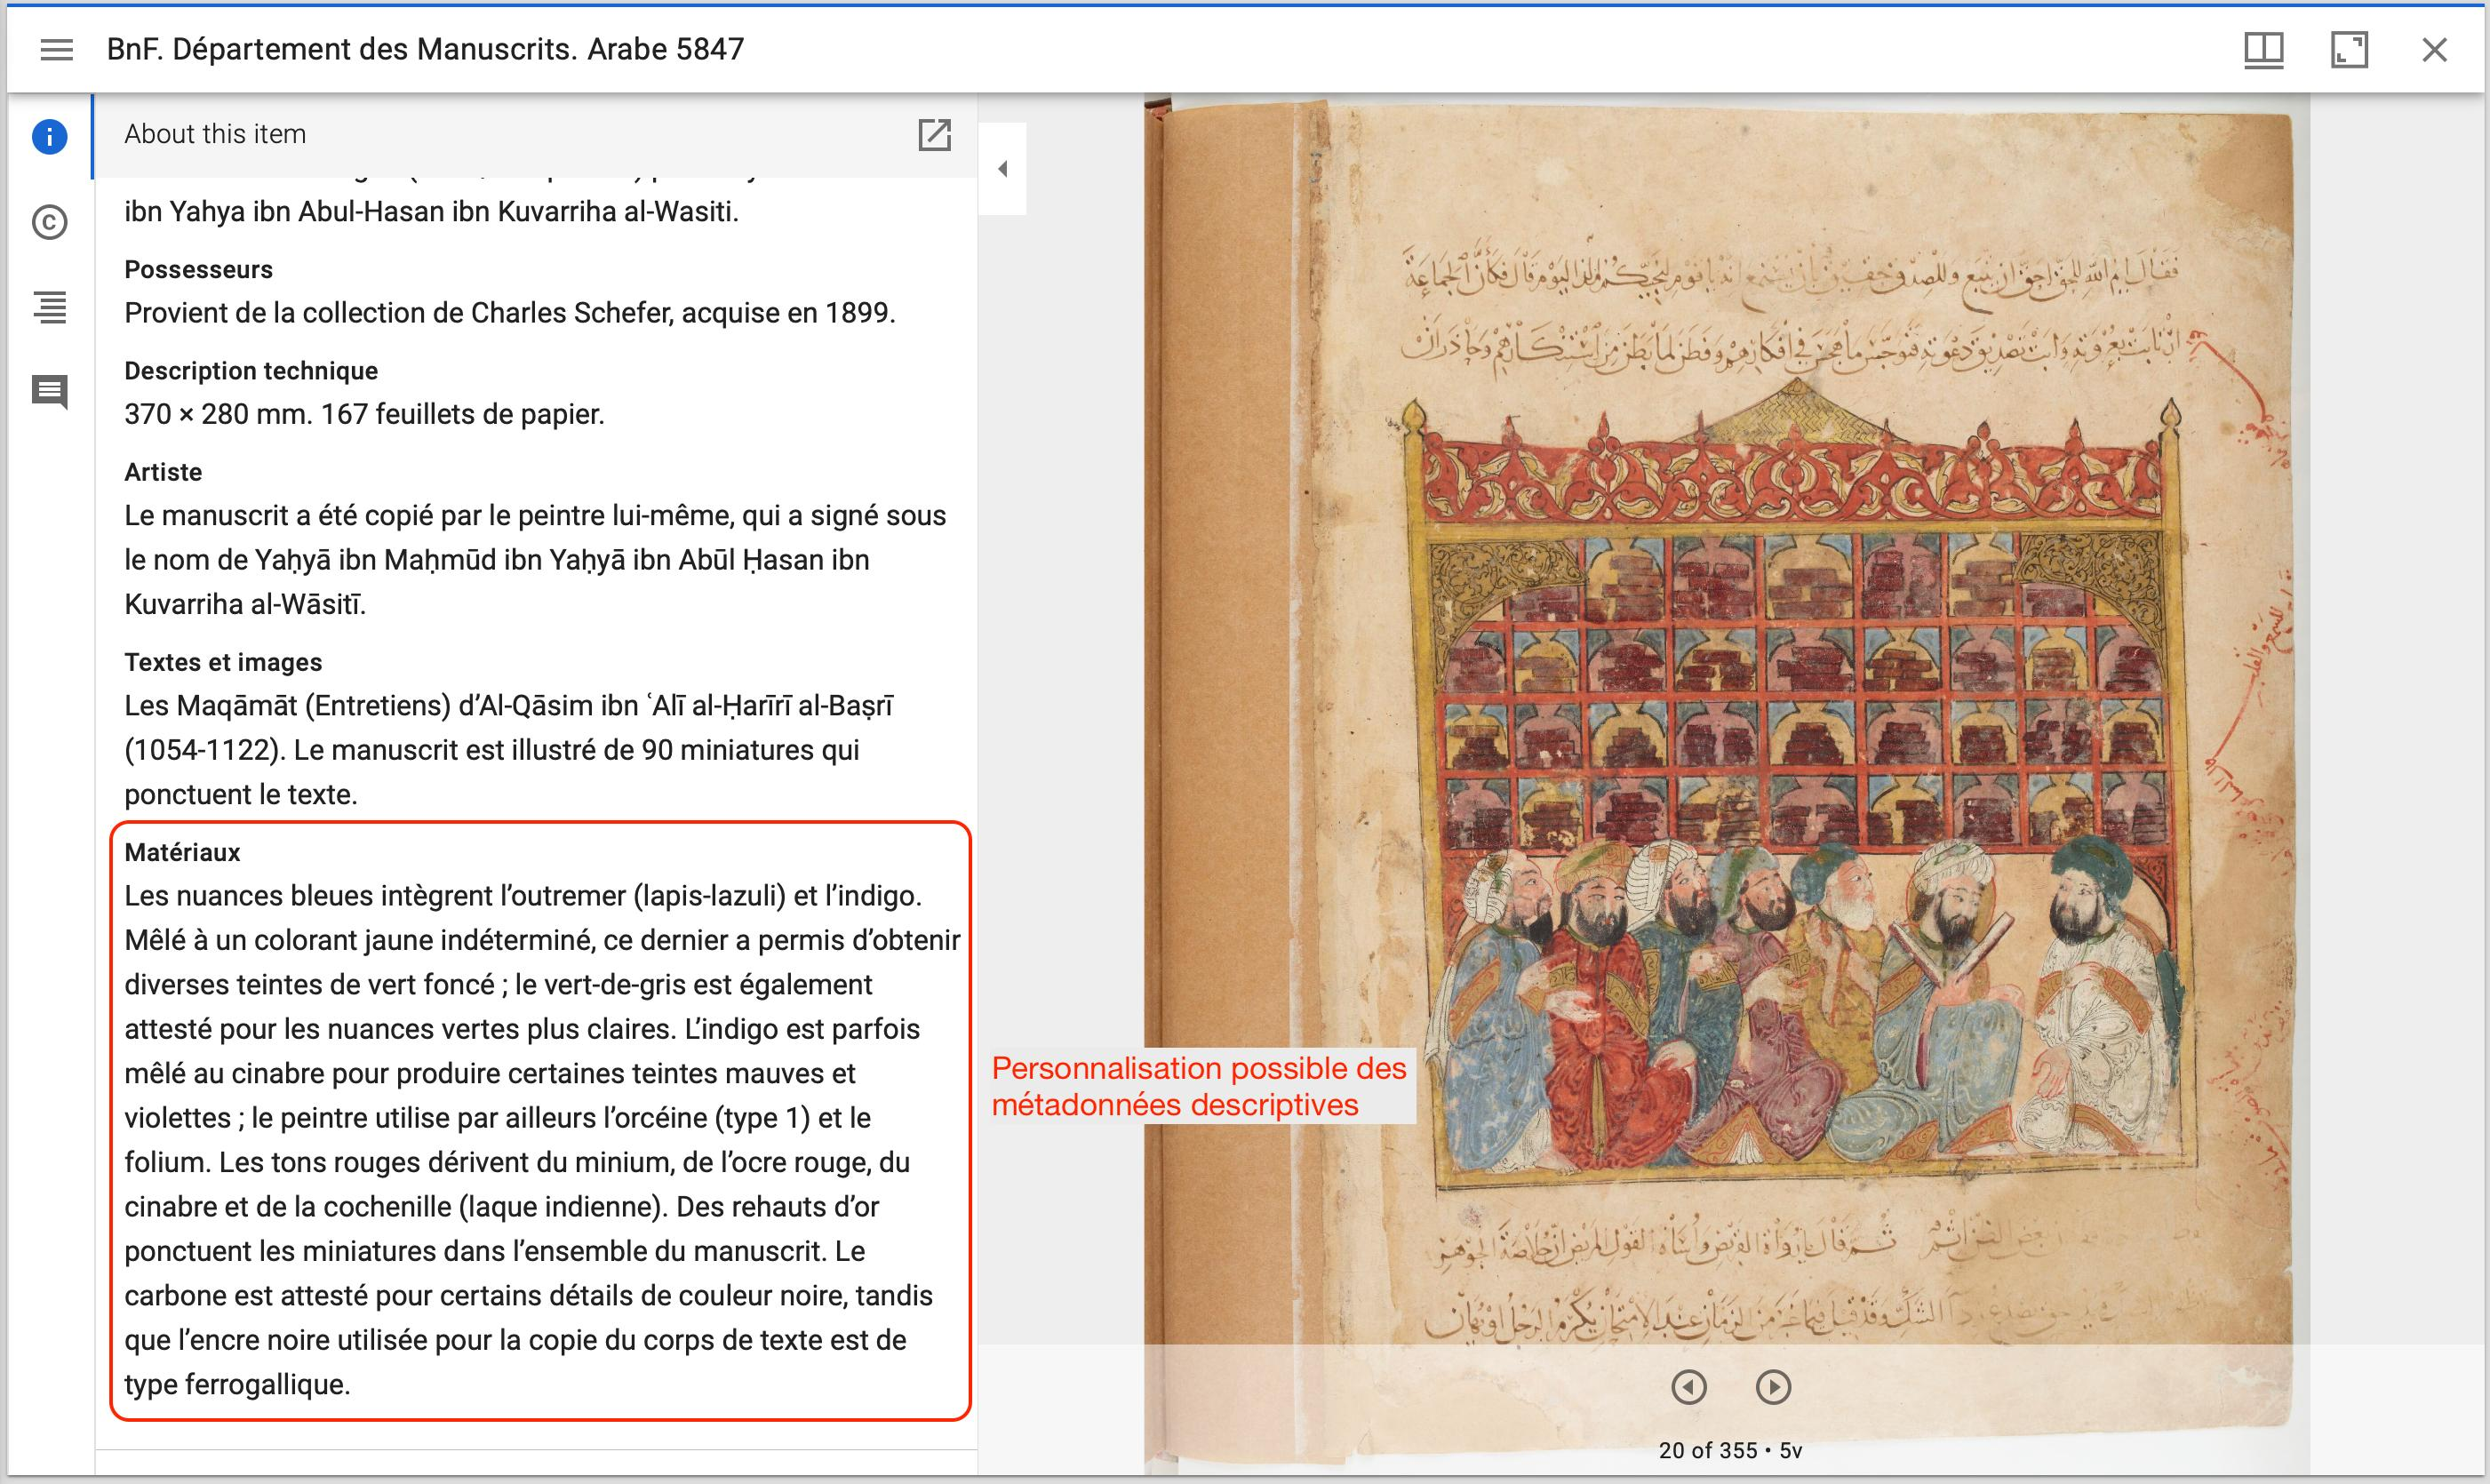
\includegraphics[width=\textwidth]{./textes/chap4/mirador-materiau.jpg}
	\caption{Personnalisation des métadonnées descriptives}
	\label{fig:info}
\end{figure}
Le fac-similé numérique peut être enrichi d’annotations\footnote{Il existe actuellement une dizaine de serveurs d’annotations IIIF. Les principales possibilités sont listées à l’adresse suivante~: https://github.com/IIIF/awesome-iiif?tab=readme-ov-file\#annotation-servers. Dans le cadre de ce stage, les annotations sont réalisées avec SimpleAnnotationServer (SAS), un serveur écrit en Java et développé par Glen Robson ( https://github.com/glenrobson/SimpleAnnotationServer).}. Ces dernières peuvent être invisibles, n’altérant pas la première lecture du manuscrit, ou visibles, permettant d’apporter des compléments d’informations. Les enrichissements possibles sur une image numérique sont nombreux. Il peut aussi bien s’agir de la transcription d’un document, d’un commentaire ou d’une analyse de contenu, ou encore de la mise en évidence d’une zone. Dans notre cas, il s’agit d’y renseigner les données de la base sur les analyses réalisées.\par
Les annotations IIIF suivent le Web Annotation Data Model\footcite{noauthor_web_2017}. Elles sont composées de deux parties. L’une renseigne le contenu de l’annotation, ce qui sera reporté sur l’image numérique~; l’autre indique la cible de l’annotation, le manifeste dont il est question et sa partie concernée par le commentaire. Une annotation simple a une structure standardisée composée de six points.\par
Structure d'une annotation~:
\begin{enumerate}
	\item @context~: il spécifie le contexte JSON-LD utilisé pour interpréter les données d'annotation.
	\item id~: un identifiant unique pour l'annotation.
	\item type~: le type de l'annotation, généralement il suffit d’indiquer "Annotation".
	\item motivation : la raison derrière l'annotation (par exemple, \enquote{commentaire}).
	\item target~: la ressource ou la partie de la ressource qui est annotée.
	\item body~: le contenu de l'annotation.
\end{enumerate}\par
De façon simplifiée, parce que celles réalisées sont finalement un peu plus complexes, une annotation sur le manuscrit Arabe 5847 peut répondre au schéma suivant~:
\begin{lstlisting}[language=json]
	{
		"@context": "http://iiif.io/api/presentation/2/context.json",
		"@id": "http://localhost:8888/annotation/1719318035104",
		"@type": "oa:Annotation",
		"motivation": ["oa:commenting"],
		"on": {
			"full": "https://gallica.bnf.fr/iiif/ark:/12148/btv1b8422965p/canvas/f34",
			"@id": "http://744902fa-f92b-4edf-b593-f9260051c14d"
		},
		"resource": {
			"chars": "<p>Motif : v&ecirc;tement, chausse dextre</p>\n<p>Couleur : rouge</p>\n<p>Mat&eacute;riau : ocre rouge</p>"
		}
	}
\end{lstlisting}

Ces annotations permettent des reports d’informations. Elles enrichissent les facs-similés numériques avec le travail réalisé lors des projets de recherche. Les données de la base, qui concernent les résultats sur les couleurs et les matériaux, peuvent être reportées et figurer directement sur les feuillets. Ainsi, le chercheur a sous les yeux les correspondances, sans avoir besoin de passer d’un document à l’autre. Mais un manifeste \indexmot{IIIF} a encore d’autres possibilités d’enrichissement qui, combinées avec les annotations, permettent de croître encore l’intérêt d’un fac-similé numérique. L’appel d’un feuillet de manuscrit pour son affichage peut être inclus dans un système de claques. Autrement dit, d’autres images numériques sont superposables à la première appelée.\par
La Bibliothèque du Congrès propose un bel exemple de l’intérêt d’une combinaison de calques avec des images \indexmot{IIIF}. Lorsqu’elle a récemment numérisé les papiers d’Alexander Hamilton, une lettre à Elizabeth Schuyler (datée du 6 septembre 1780, deux mois avant leur mariage), non éditée, avec quatorze lignes effacées par l’auteur, est devenue visible pour la première fois. Pour savoir ce qui se trouvait sous les rayures, la Bibliothèque du Congrès a utilisé l'imagerie hyperspectrale. Une analyse non invasive qui utilise la lumière à différentes longueurs d'onde pour capturer des informations non visibles à l'œil. Cette technologie a permis de révéler le contenu. La bibliothèque a réalisé un manifeste \indexmot{IIIF} de la lettre, pour permettre aux utilisateurs d’en découvrir la teneur par eux-mêmes en jouant sur le niveau d’opacité des calques\footnote{https://dvp.prtd.app/hamilton/manifest.json}.
\begin{figure}[H]
	\centering
	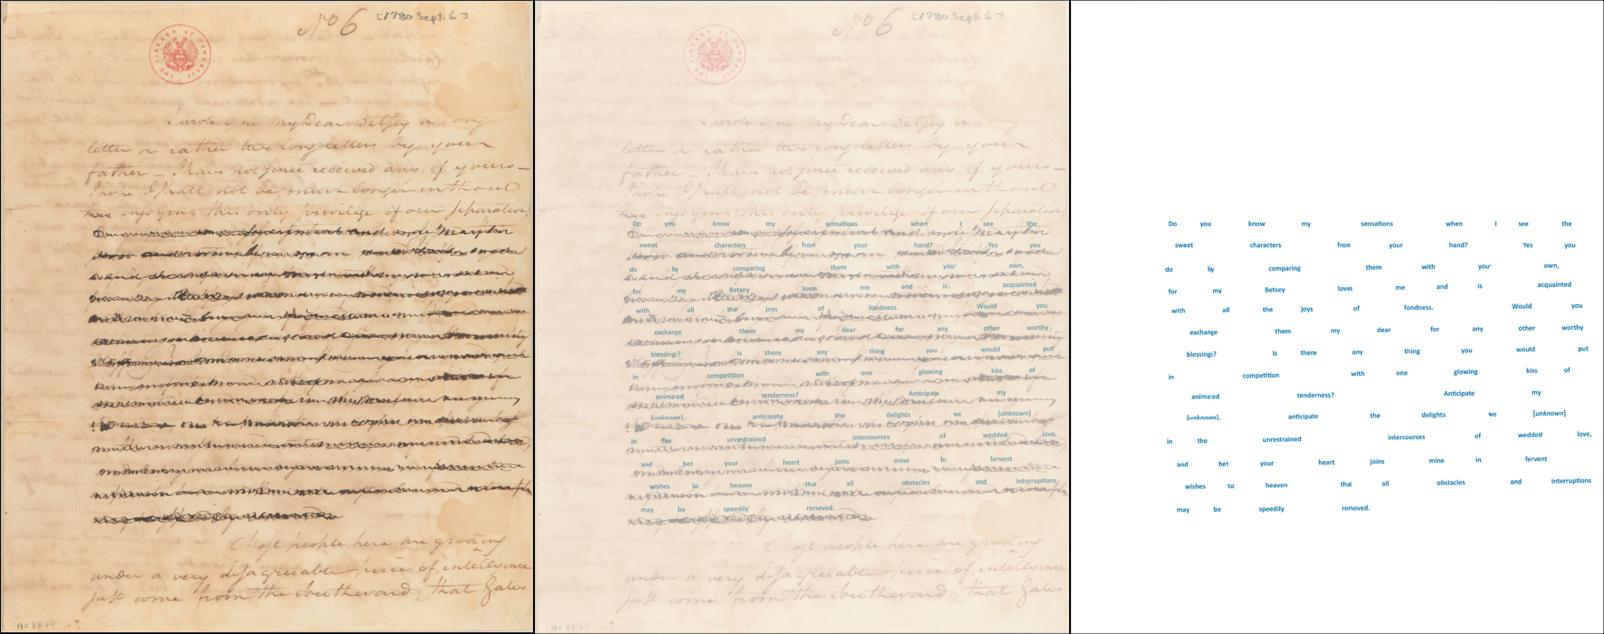
\includegraphics[width=\textwidth]{./textes/chap4/iiif-calque.jpg}
	\caption{Lettre d'Alexander Hamilton}
	\label{fig:info}
\end{figure}
Le projet de recherche \enquote{La couleur~: artefacts, matière et cognition} possède également des images numériques issues d’analyses hyperspectrales. Les laboratoires en charge des rapports d’analyses physico-chimiques ont fourni, au moment de leurs résultats, des doubles numériques au commanditaire. Il est ainsi possible d’envisager, à l’image de ce qu’a proposé la Bibliothèque du Congrès, de réaliser des claques sur les feuillets de manuscrit, permettant de découvrir les images hyperspectrales correspondantes et donc les résultats.\newpage

\section{La sélection du département des manuscrits}

Le fac-similé numérique produit est considérablement enrichi au regard de simples reproductions numériques d’images habituellement disponibles. Douze manuscrits ont fait l’objet d’une transformation en manifeste \indexmot{IIIF}\footnote{Les liens des manifestes \indexmot{IIIF} sont reportés en annexe.}. Ils sont retenus en raison de la qualité exceptionnelle de leurs enluminures. Une fois les sites Omeka~S accessibles au public, ils constitueront une petite sélection pour les utilisateurs, un modèle du travail effectué au cours des années du projet de recherche.\\\par
\begin{tabular}{>{\raggedright}p{0.5cm} >{\raggedright\arraybackslash}p{14cm}}
	1. & Le Psautier de Paris (BnF. Département des Manuscrits. Grec 139) \\[10pt]
	2. & L’Evangéliaire dit de Charlemagne ou de Godescalc (BnF. Département des Manuscrits. NAL 1203) \\[10pt]
	3. & Le Beatus a Liebana, Commentarius in Apocalypsin (BnF. Département des Manuscrits. Latin 8878) \\[10pt]
	4. & Les Evangiles dits d'Echternach ou de Saint Willibrord (BnF. Département des Manuscrits. Latin 9389) \\[10pt]
	5. & L’Ancien Testament et quelques feuillets du Nouveau Testament en syriaque (BnF. Département des Manuscrits. Syriaque 341) \\[10pt]
	6. & Le Tétraévangile (BnF. Département des Manuscrits. Copte 13) \\[10pt]
	7. & Les Makamat de Hariri (BnF. Département des Manuscrits. Arabe 5847) \\[10pt]
	8. & Le Codex Xolotl (BnF. Département des Manuscrits. Mexicain 1-10) \\[10pt]
	9. & L’Évangéliaire dit de Poussay (BnF. Département des Manuscrits. Latin 10514) \\[10pt]
	10. & Le Codex Sinopensis (BnF. Département des Manuscrits. Supplément Grec 1296) \\[10pt]
	11. & Le Psautier dit de saint Louis (BnF. Département des Manuscrits. Latin 10525) \\[10pt]
	12. & Un recueil d'œuvres en prose et en vers, probablement toutes dues à Naṣīr al-Dīn Muḥ. b. Ibrāhīm b. ʿAbd-ullāh al-Rammāl al-Muʿazzim al-Sāʿatī al-Haykalī (BnF. Département des Manuscrits. Persan 174) \\[10pt]
\end{tabular}

Les manuscrits sont tous enrichis de métadonnées descriptives. Ils offrent une première approche avec le manuscrit dans une courte introduction, puis quelques phrases qui retracent son historique, suit ensuite une petite fiche technique, puis un commentaire sur le texte et les images, une note sur le ou les artistes et, enfin, quelques grandes lignes sur les matériaux découverts lors des analyses. \par
Ci-dessous, l’exemple de la présentation du manuscrit Latin 10514 telle que visible dans Mirador~:\par

\begin{mdframed}[style=graybox]
	LIBELLÉ~:\par
	BnF. Département des Manuscrits. Latin 10514\par
	DESCRIPTION~:\par
	Évangéliaire dit de Poussay\par
	INTRODUCTION~:\par
	Réalisé dans l’abbaye de Reichenau à la fin du Xe siècle, vers 980, l’Évangéliaire de Poussay fait partie du groupe des manuscrits dit \enquote{de Ruodprecht}, d’après le copiste du Psautier d’Egbert, également originaire de Reichenau. Il s’agit d’un évangéliaire festif contenant des enluminures sur fond pourpre. Sa destination est incertaine, mais il a été offert vers 1036 à l’abbaye de Poussay par Brunon d’Eguisheim-Dagsbourg, alors évêque de Toul et devenu pape entre 1049-1054 sous le nom de Léon~IX.\par
	POSSESSEURS~:\par
	Trésor de l’abbaye de Poussay jusqu’à la Révolution française (?)~; bibliothèque de la Ville de Mirecourt~; acquis en 1844 par la Bibliothèque royale contre des livres imprimés.\par
	DESCRIPTION TECHNIQUE~:\par
	285 x 205 mm 133 feuillets de parchemin\par
	TEXTES ET IMAGES~:\par
	13 peintures en pleine page~: f.~3v Ecclésiastique offrant son livre, conduit par 2 anges~; f.~4r Christ trônant, main étendue vers le donateur~; f.~5v saint Luc inspiré par le bœuf~; f.~6r saint Marc inspiré par le lion~; f.~7v saint Jean examinant sa plume~; f.~8r saint Matthieu écrivant~; f.~9v Nativité~; f.~18v Adoration des mages~; f.~35v crucifixion~; f.~46v le lavement des pieds~; f.~50v deux saintes femmes au Tombeau~; f.~66v Ascension~; f.~69v Pentecôte~; 16 pages d’initia ornées~: f.~10r~; f.~13r~; f.~19r~; f.~25r~; f.~36r~; f.~49r~; f.~51r~; f.~67r; f.~70r~; f.~81r~; f.~84r~; f.~95r~; f.~97r~; f.~102r~; f.~119r~; 7~pages d’incipit ornées~: f.~12v~; f.~48v~; f.~80v~; f.~94v ~; f.~96v~; f.~101v~; f.~118v.\par
	ARTISTES~:\par
	Le décor est de la main d’un seul artiste, dont le style se caractérise par la monumentalité des personnages représentés et la densité de certaines compositions. Son style a été rapproché de celui du Psautier d’Egbert (Cividale, Museo Archaeologico Nazionale, cod. 136) qui fut évêque de Trèves à partir de 977.\par
	MATÉRIAUX~:\par
	Les fonds des enluminures à pleines pages sont pourprés. La palette utilisée est large mais délimitée~: rouge, vert, jaune, doré, violet, des touches de bleus et des nuances de bruns et de gris. Le bleu est réalisé à partir d’outremer (lapis-lazuli)~; les tons de rouge, de violet et parfois de brun contiennent de l’orseille, pigment obtenu à partir de lichen, mélangé parfois avec de l’oxyde de plomb pour le marron. Le jaune contient de l’ocre jaune, qui est associé au vert-de-cuivre pour obtenir les teintes de couleur verte.\\\par
\end{mdframed}

En deuxième lieu, les manifestes sont annotés selon les points d’analyses qui sont renseignés dans les données de la base. Il faut faire un choix pour le commentaire des annotations, trois informations sont retenues~: le motif analysé, la couleur et les matériaux découvert. Ces trois données sont celles qui correspondent le mieux au principe de l’annotation, puisqu’elles concernent des points d’analyses précis, là où d’autres concernent le feuillet ou le manuscrit. Si je reprends le cas du manuscrit Latin 9389, les informations de la base sont reportées selon le modèle ci-dessous, à gauche. Seuls les commentaires du Latin 8878 ont une autre présentation, comme visible à droite.\par
\begin{figure}[H]
	\centering
	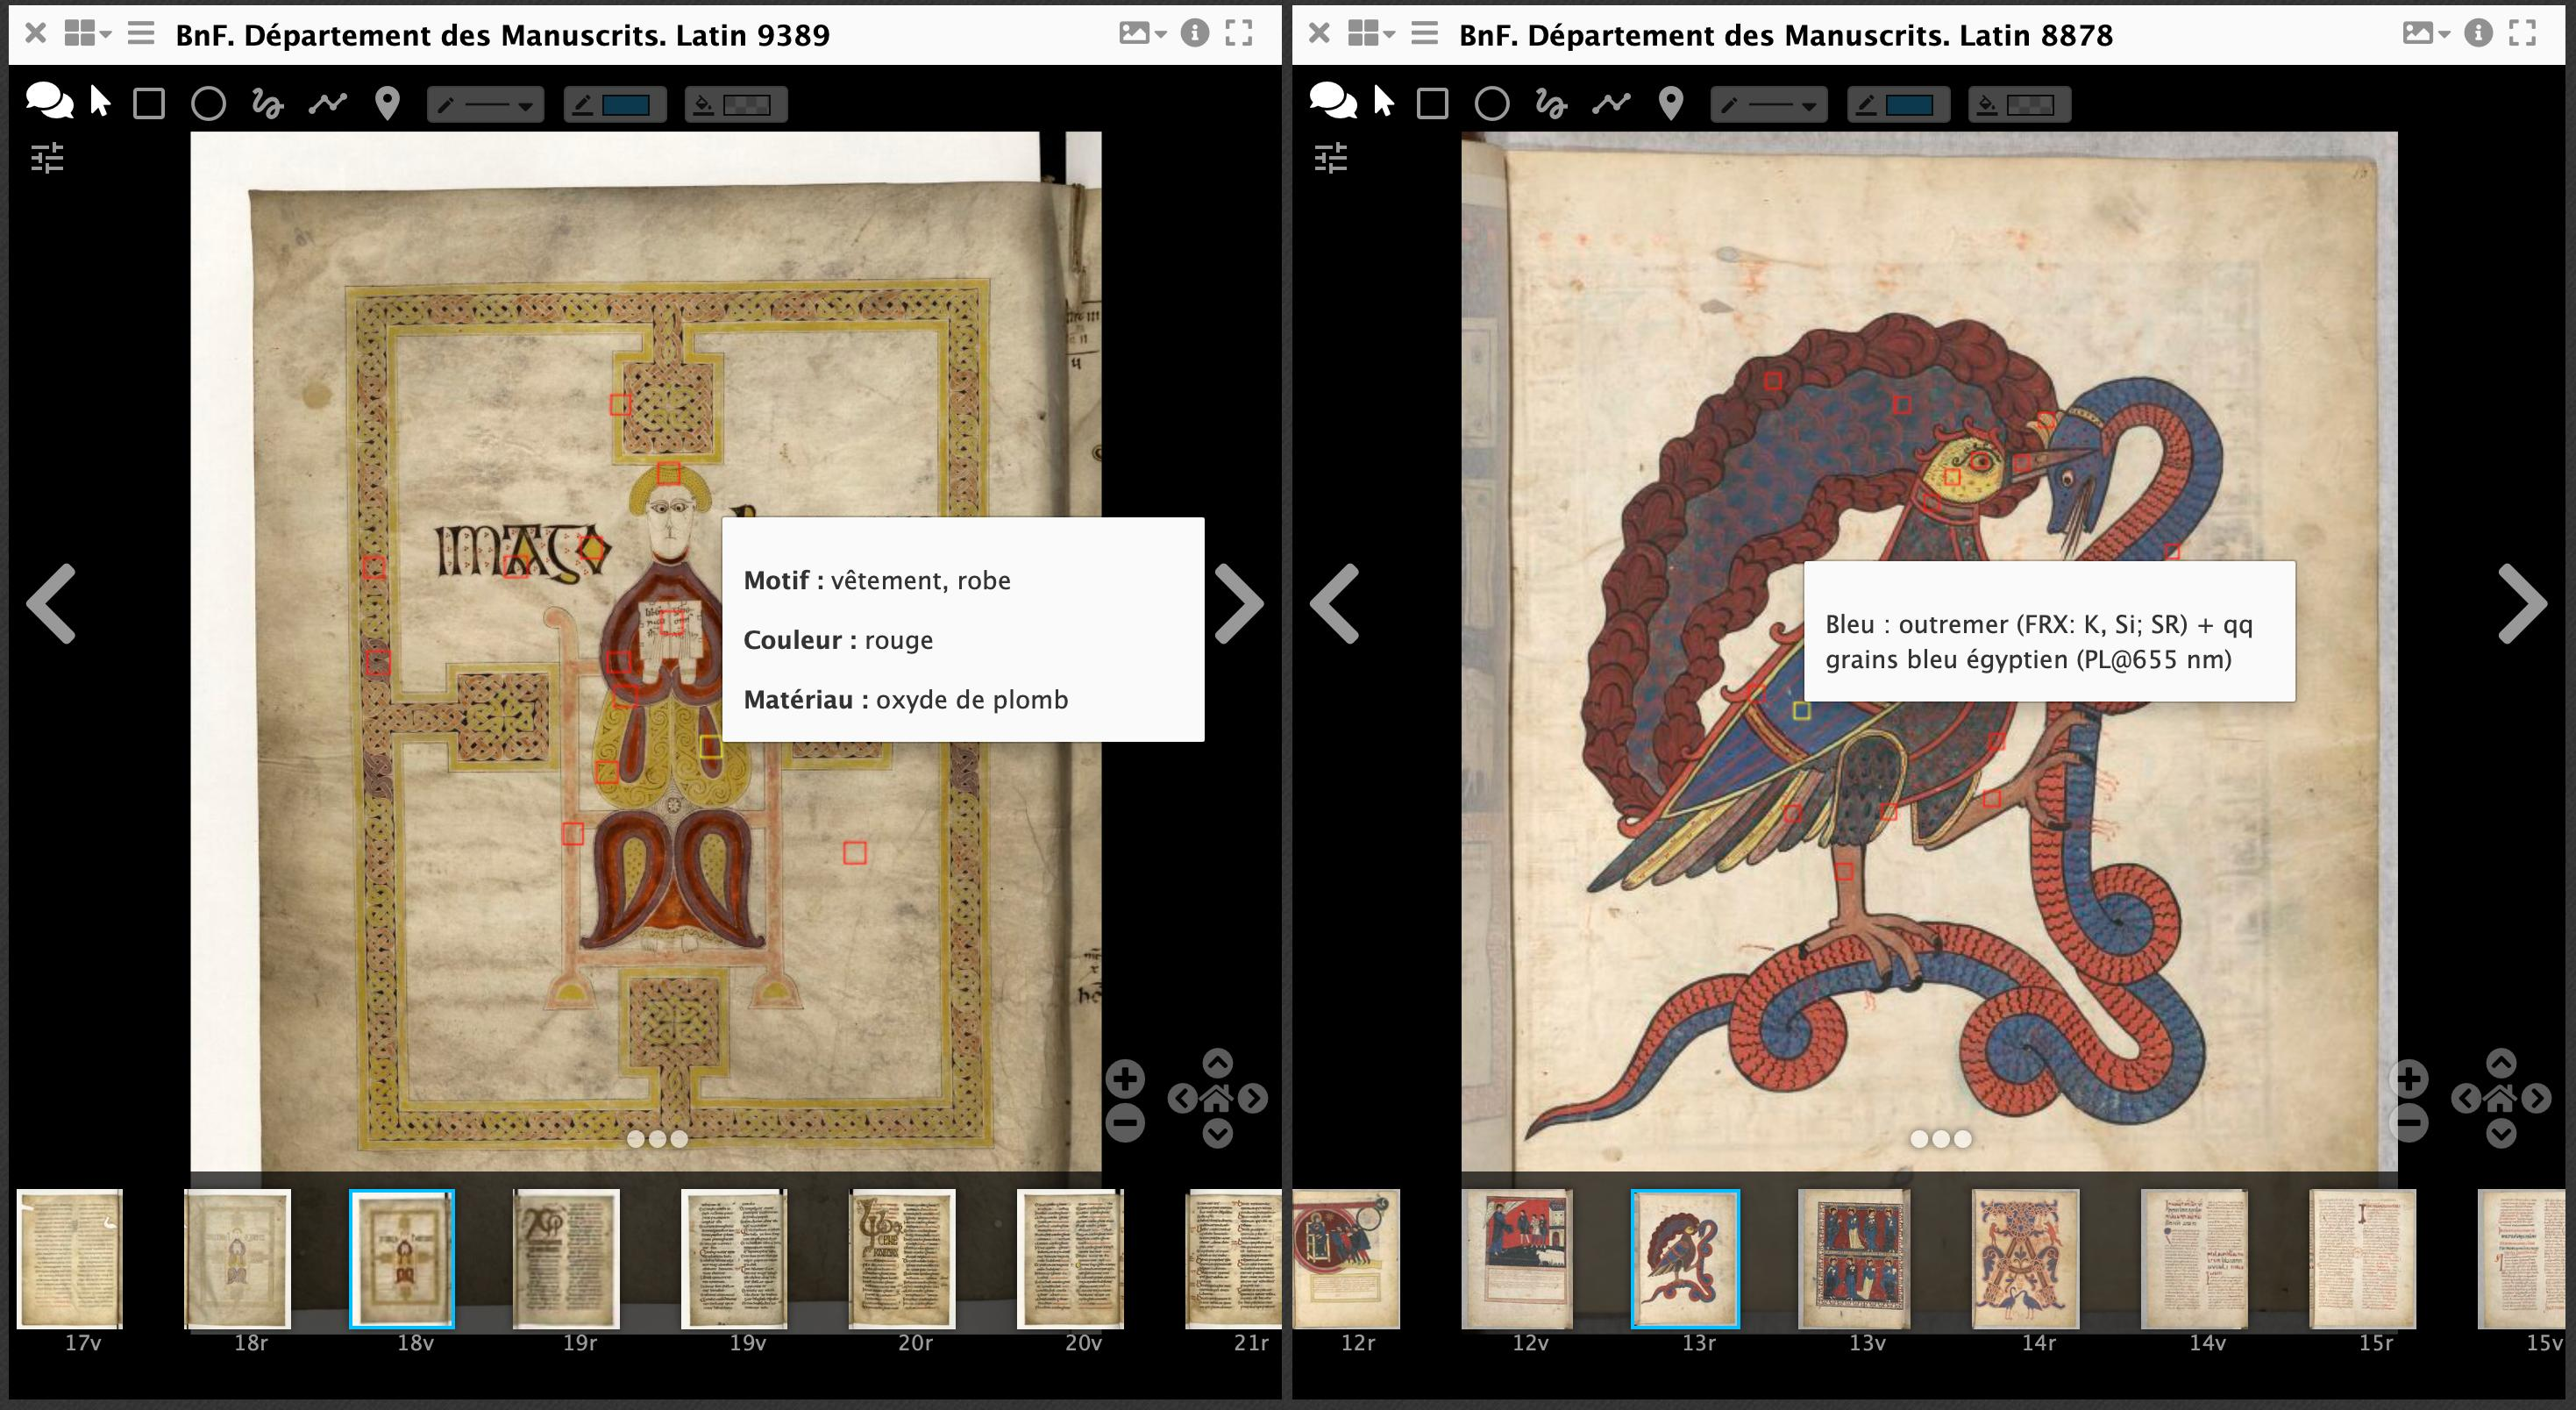
\includegraphics[width=\textwidth]{./textes/chap4/iiif-annot.jpg}
	\caption{Annotations dans Mirador}
	\label{fig:info}
\end{figure}
Enfin, un système de calque vient mettre en complément de l’image numérique du feuillet les résultats obtenus par les analyses hyperspectrales. Ils sont invisibles au chargement de la page, mais ils apparaissent une fois sélectionnés dans la barre latérale. L’affichage sous Mirador permet de cumuler l’affichage des calques à celles des annotations. Ainsi, il est permis d’additionner les résultats de différentes analyses pour avoir toutes les informations nécessaires sur le feuillet en question.\par
\begin{figure}[H]
	\centering
	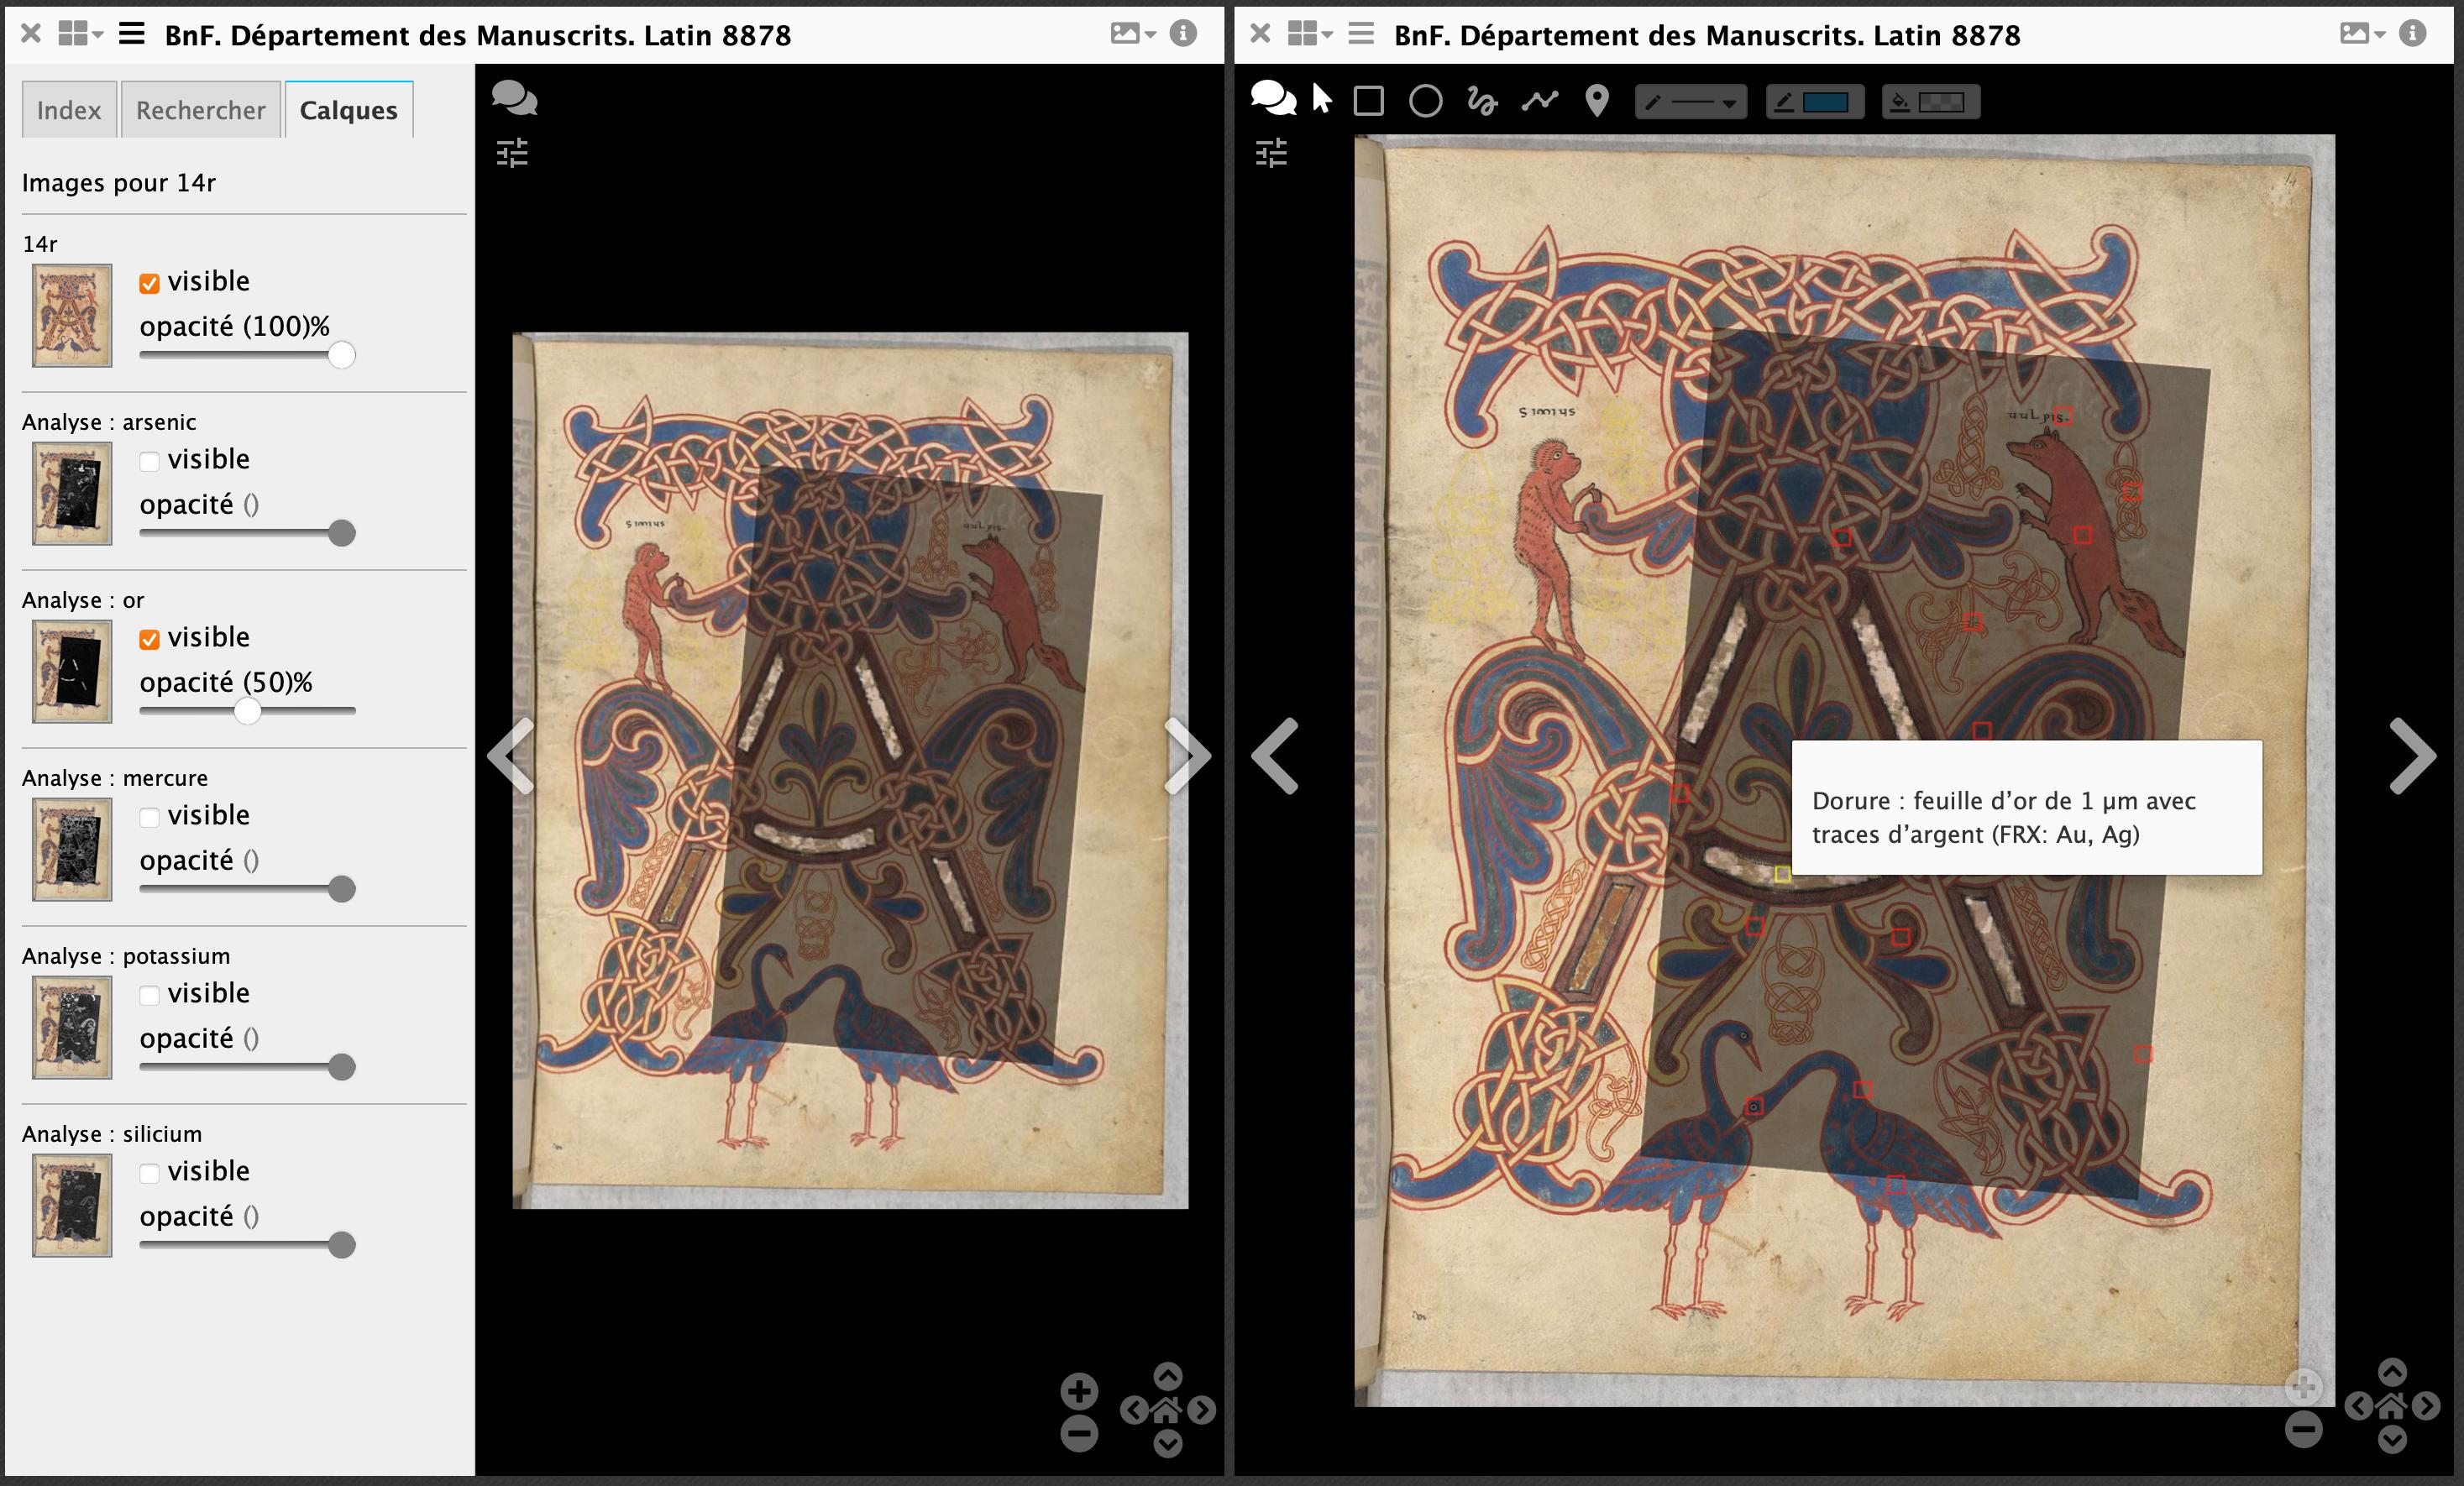
\includegraphics[width=\textwidth]{./textes/chap4/iiif-calque-annot.jpg}
	\caption{Addition d'un calque et d'une annotation}
	\label{fig:info}
\end{figure}
Un fac-similé de cette nature facilite la communication et la médiation de la recherche. Les chercheurs ont à leur disposition les images numériques en haute résolution des feuillets, la présentation du manuscrit, ainsi que le résultat des analyses menées dans le cadre du projet de recherche. Les données de la base sont à la disposition du public, mais elles sont également intelligibles parce que contextualisées sur la source même du travail. Elles ne sont plus inscrites dans des CSV à plusieurs milliers de lignes, mais sur l’objet même de la recherche. \par
Le fac-similé numérique permet aussi d’instaurer un langage commun entre des cultures scientifiques diverses. Ainsi, le scientifique et les historiens, historiens de l’art, spécialistes des textes anciens ont sous les yeux le document qui est l’objet de leur discussion. Ils peuvent y rapporter directement leurs commentaires, leurs analyses et leurs résultats. Des étapes de traductions scientifiques, qui peuvent être parfois à la source d’erreurs, non plus lieu d’être et les processus de communication sont simplifiés.\newpage

*\\\par
Le projet détaillé ici n’a pu trouver son aboutissement dans le cadre de ce stage. Les deux projets scientifiques sont hébergés à partir de l’automne sur un site Omeka~S. En conséquence, et en anticipation de la migration, un essai d’implémentation d’une visionneuse dans Omeka~S\footnote{Pour l’implémentation de Mirador dans Omeka S, voir annexe 3.} a été réalisé. Cet essai a également pour objectif de s’assurer de la bonne conformité des manifestes~\indexmot{IIIF} précédemment cités. Cependant, il s’est avéré que le module Mirador proposé pour Omeka est appauvri par rapport aux versions de la visionneuse qui peuvent être trouvées sur le web. Si une solution a été trouvée pour la gestion des annotations, il n’en est pas de même pour les calques d’images\footnote{Cf annexe 4.}. Les manifestes qui seront proposés à l’automne sur les sites Omeka~S ne proposeront donc pas ce dernier enrichissement pour les fac-similés. Néanmoins, les facs-similés numériques produits demeurent de nouveaux outils de recherche mis à la disposition du public et utiles pour la communication de la recherche. 